\documentclass[11pt]{article}
\usepackage{certmachine}
\usepackage{graphicx}
%% generated by tools/paper-numbers/erdos1038-sup.js from certs/sublevel-tao179.json, the sublevel instrument, the sublevel battery and the lemniscate verifier (run live) — do not edit (git 054078d19462)
\newcommand{\RepoCommit}{054078d19462}
\newcommand{\RecDate}{2026-09-01}
\newcommand{\RecGit}{cd057d7}
\newcommand{\RecMinutes}{48.1}
\newcommand{\TwoSqrtTwo}{2.8284271247}
\newcommand{\TwoSqrtTwoD}{2.8284271}
\newcommand{\TOddFrac}{141/50}
\newcommand{\TOdd}{2.82}
\newcommand{\TEvenFrac}{56569/20000}
\newcommand{\TEven}{2.82845}
\newcommand{\GapOdd}{0.0084}
\newcommand{\GapOddSci}{$8.43\times10^{-3}$}
\newcommand{\SlackEven}{$2.29\times10^{-5}$}
\newcommand{\NTheorems}{6}
\newcommand{\NTheoremsWord}{six}
\newcommand{\OddDegrees}{3, 5, 7}
\newcommand{\EvenDegrees}{4, 6, 8}
\newcommand{\MaxDegree}{8}
\newcommand{\BoxesThree}{127}
\newcommand{\LeavesThree}{45}
\newcommand{\DepthThree}{16}
\newcommand{\SecondsThree}{0.01}
\newcommand{\BoxesFour}{549}
\newcommand{\LeavesFour}{213}
\newcommand{\DepthFour}{59}
\newcommand{\SecondsFour}{0.06}
\newcommand{\BoxesFive}{1{,}583}
\newcommand{\LeavesFive}{522}
\newcommand{\DepthFive}{37}
\newcommand{\SecondsFive}{0.21}
\newcommand{\BoxesSix}{4{,}219}
\newcommand{\LeavesSix}{1{,}370}
\newcommand{\DepthSix}{89}
\newcommand{\SecondsSix}{0.65}
\newcommand{\BoxesSeven}{28{,}773}
\newcommand{\LeavesSeven}{9{,}472}
\newcommand{\DepthSeven}{63}
\newcommand{\SecondsSeven}{8.8}
\newcommand{\BoxesEight}{31{,}425}
\newcommand{\LeavesEight}{9{,}330}
\newcommand{\DepthEight}{118}
\newcommand{\SecondsEight}{5.7}
\newcommand{\TotalBoxes}{66{,}676}
\newcommand{\TotalLeaves}{20{,}952}
\newcommand{\TotalSeconds}{15}
\newcommand{\TheoremRows}{$3$ & $\sup_{3} < 2.82$ & $141/50$ & 127 & 45 & 16 & 0.01 & strict \\
$4$ & $\sup_{4} \in [2\sqrt2,\ 2.82845]$ & $56569/20000$ & 549 & 213 & 59 & 0.06 & localized \\
$5$ & $\sup_{5} < 2.82$ & $141/50$ & 1{,}583 & 522 & 37 & 0.21 & strict \\
$6$ & $\sup_{6} \in [2\sqrt2,\ 2.82845]$ & $56569/20000$ & 4{,}219 & 1{,}370 & 89 & 0.65 & localized \\
$7$ & $\sup_{7} < 2.82$ & $141/50$ & 28{,}773 & 9{,}472 & 63 & 8.8 & strict \\
$8$ & $\sup_{8} \in [2\sqrt2,\ 2.82845]$ & $56569/20000$ & 31{,}425 & 9{,}330 & 118 & 5.7 & localized \\}
\newcommand{\RefusedDegree}{9}
\newcommand{\RefusedWhy}{bnb: box budget exhausted}
\newcommand{\RefusedMinutes}{47.9}
\newcommand{\RefusedBudgetBoxes}{1{,}500{,}000}
\newcommand{\RefusedBudgetDepth}{160}
\newcommand{\BudgetRows}{$3$ & 500{,}000 & 40 \\
$5$ & 3{,}000{,}000 & 70 \\
$7$ & 5{,}000{,}000 & 100 \\
$4$ & 3{,}000{,}000 & 120 \\
$6$ & 3{,}000{,}000 & 160 \\
$8$ & 1{,}500{,}000 & 200 \\
$9$ & 1{,}500{,}000 & 160 \\}
\newcommand{\WitnessEnclosure}{[2.828427124745,\ 2.828427124747]}
\newcommand{\WitnessWidth}{$1.1\times10^{-12}$}
\newcommand{\WitnessLoFrac}{7774721279937/2748779069440}
\newcommand{\WitnessHiFrac}{388736063997/137438953472}
\newcommand{\CalibrationRows}{$x^2-1$ & $[2.828427124745,\ 2.828427124747]$ & $2\sqrt2$ & 3 \\
$x^2$ & $[1.999999999999,\ 2.000000000001]$ & $2$ & 2 \\
$x$ & $[1.999999999999,\ 2.000000000001]$ & $2$ & 2 \\
$(x-1)^2$ & $[1.999999999999,\ 2.000000000001]$ & $2$ & 2 \\
$(x^2-1)^2$ & $[2.828427124745,\ 2.828427124747]$ & $2\sqrt2$ & 3 \\}
\newcommand{\SweepRows}{$3$ & $8$ & 505 & $(-1,\ 3/4,\ 1)$ & $[2.744632,\ 2.744633]$ \\
$4$ & $4$ & 264 & $(-1,\ -1,\ 1,\ 1)$ & $[2.828427,\ 2.828428]$ \\
$5$ & $2$ & 69 & $(-1,\ -1,\ 1/2,\ 1,\ 1)$ & $[2.747268,\ 2.747269]$ \\}
\newcommand{\SweepConfigs}{838}
\newcommand{\CubicRoot}{201/256}
\newcommand{\CubicRootD}{0.7852}
\newcommand{\CubicChampion}{[2.754173,\ 2.754174]}
\newcommand{\CubicChampionLo}{2.754173}
\newcommand{\CubicChampionHi}{2.754174}
\newcommand{\QuinticRoot}{905/1024}
\newcommand{\QuinticRootD}{0.8838}
\newcommand{\QuinticPeak}{[2.801090,\ 2.801091]}
\newcommand{\QuinticPeakLo}{2.801090}
\newcommand{\QuinticPeakHi}{2.801091}
\newcommand{\QuinticRuns}{1}
\newcommand{\GapThreeToTOdd}{0.0658}
\newcommand{\GapFiveToTOdd}{0.0189}
\newcommand{\CubicGridMaxR}{100/128}
\newcommand{\CubicGridMax}{2.753089}
\newcommand{\QuinticGridMaxR}{3620/4096}
\newcommand{\QuinticGridMax}{2.801091}
\newcommand{\SplitBeforeR}{3620/4096}
\newcommand{\SplitBeforeV}{2.801091}
\newcommand{\SplitAfterR}{3622/4096}
\newcommand{\SplitAfterV}{2.798779}
\newcommand{\SplitGapLo}{-0.2177}
\newcommand{\SplitGapHi}{-0.2153}
\newcommand{\SplitGapWidth}{0.002}
\newcommand{\SplitDrop}{0.002}
\newcommand{\FineLastR}{3664/4096}
\newcommand{\FineLastV}{2.686190}
\newcommand{\FineLastGapWidth}{0.117}
\newcommand{\FineStep}{1/4096}
\newcommand{\FineFrom}{3600/4096}
\newcommand{\FineTo}{3664/4096}
\newcommand{\CubicSplitR}{101/128}
\newcommand{\CubicSplitV}{2.726610}
\newcommand{\CubicEndV}{2.205570}
\newcommand{\QuinticEndV}{2.436924}
\newcommand{\CurvePoints}{163}
\newcommand{\InfBracketLo}{1.828}
\newcommand{\InfBracketHi}{1.8344304971959906}
%% InfUpperAboveD is defined after the verifier runs
\newcommand{\BatteryChecks}{6}
\newcommand{\BatteryReds}{3}
\newcommand{\BatteryMs}{76}
\newcommand{\VerPassed}{26}
\newcommand{\VerFailed}{0}
\newcommand{\VerMutations}{4}
\newcommand{\VerNamed}{22}
\newcommand{\VerMs}{58}
\newcommand{\KrawczykRounds}{1}
\newcommand{\KrawczykRad}{$3.84\times10^{-14}$}
\newcommand{\WidthQ}{$1.64\times10^{-45}$}
\newcommand{\WidthU}{$3.18\times10^{-45}$}
\newcommand{\WidthV}{$1.12\times10^{-45}$}
\newcommand{\WidthWorst}{$3.18\times10^{-45}$}
\newcommand{\DForty}{1.8344304757626617110907536351247861430208}
\newcommand{\InfUpperAboveD}{$2.14\times10^{-8}$}
\newcommand{\DPrintedThirty}{1.834430475762661711090753635125}
\newcommand{\DTwentyNine}{1.83443047576266171109075363512}
\newcommand{\DPrintedLastDigit}{5}
\newcommand{\DExpansionThirtieth}{4}
\newcommand{\DExpansionTail}{47861}
\newcommand{\ClaimRows}{$D$ & p.2 & $1.834430475762661711090753635125$ & $1.834430475762661711090753635124786\ldots$ & rounded \\
$\alpha$ & p.5 & $0.804461754260998666$ & $0.804461754260998666841\ldots$ & truncation \\
$q^*$ & p.24 & $0.949858345823470318$ & $0.949858345823470318483\ldots$ & truncation \\
$u^*$ & p.24 & $0.893966122075456116$ & $0.893966122075456116111\ldots$ & truncation \\
$v^*$ & p.24 & $0.964555096995821406$ & $0.964555096995821406396\ldots$ & truncation \\
$p^*$ & p.24 & $0.824521729252520379$ & $0.824521729252520379285\ldots$ & truncation \\
$\alpha$ & p.24 & $0.804461754260998666$ & $0.804461754260998666841\ldots$ & truncation \\
$r^*$ & p.24 & $0.0263231076477328506$ & $0.0263231076477328506351\ldots$ & truncation \\
$z^*$ & p.24 & $-1.808107368114928860$ & $-1.808107368114928860455\ldots$ & truncation \\
$D$ & p.24 & $1.834430475762661711$ & $1.834430475762661711090\ldots$ & truncation \\}
\newcommand{\CentreRows}{$q_0$ & $0.94985834582347031848349802544031979$ & $0.94985834582347031848349802544031979\ldots$ \\
$u_0$ & $0.89396612207545611611103128550805002$ & $0.89396612207545611611103128550805002\ldots$ \\
$v_0$ & $0.96455509699582140639698562612728156$ & $0.96455509699582140639698562612728156\ldots$ \\}
\newcommand{\CentreDecimals}{35}
\newcommand{\FaceRLo}{$4.05\times10^{-30}$}
\newcommand{\FaceRHi}{$6.42\times10^{-30}$}
\newcommand{\FaceLLo}{$7.84\times10^{-29}$}
\newcommand{\FaceLHi}{$9.04\times10^{-29}$}
\newcommand{\RadiusI}{10^{-31}}
\newcommand{\RadiusB}{10^{-30}}
\newcommand{\MarginDecades}{14}
\newcommand{\MutTwo}{1.307}
\newcommand{\MutThree}{$1.19\times10^{-9}$}
\newcommand{\MutFour}{$-4.78\times10^{-10}$}


\newcommand{\dist}{\operatorname{dist}}
\newcommand{\meas}[1]{\lvert #1 \rvert}

\title{The supremum side of Erd\H{o}s problem \#1038:\\
per-degree certificates for the $2\sqrt2$ bound,\\
and the thirty published decimals of the infimum verified}
\author{\cmauthor}
\date{October 2026 --- draft v0.1 for review; every number interpolated from the record; machine-derived, not peer-reviewed; author list to be agreed}

\begin{document}
\maketitle

\begin{abstract}
Erd\H{o}s, Herzog and Piranian asked for the infimum and the supremum of the Lebesgue measure of
$\{x\in\R:\abs{f(x)}<1\}$ over monic polynomials $f$ with all roots in $[-1,1]$. The supremum is
$2\sqrt2$, attained by $x^2-1$; in December 2025 Tao reformulated the problem over probability
measures on $[-1,1]$ and proved the supremum there, with the two-atom measure as the only
case of equality. Weights with denominator $N$ are exactly the root measures of degree-$N$
polynomials, so the statement has a decidable instance at every degree. This paper records
such decisions, made in exact arithmetic and sharing nothing with the potential-theoretic
proof: for degrees $\OddDegrees$ every polynomial has sublevel measure below $\TOdd$, a margin
of $\GapOdd$ under $2\sqrt2$ that the theorem does not state; for degrees $\EvenDegrees$ the
degree supremum is placed in $[2\sqrt2,\TEven]$ with the witness $(x^2-1)^{N/2}$ at the left end,
an enclosure weaker than the theorem by \SlackEven; degree $\RefusedDegree$ exhausted its box
budget and is recorded as refused. The certificates are branch-and-bound trees over root boxes,
$\TotalBoxes$ boxes in all, pruned by a product-of-distances bound whose own sublevel measure is
computed by the same certified Sturm machinery. Certified landscape data show the cubic maximum
at an interior root, $r=\CubicRoot$, and both families losing an interior interval of their
sublevel set past their champion. Separately, the thirty decimals of the infimum constant
$D=\DPrintedThirty\ldots$ printed in the July 2026 manuscript of Darvas, Peng and Tao are decided
against an enclosure of width below $10^{-40}$ obtained by a Krawczyk argument: every printed
constant is correct, and the thirtieth decimal is a half-up rounding of an expansion that
continues $\ldots\DExpansionTail\ldots$.
\end{abstract}

\section{Introduction}

\paragraph{The problem.}
For a non-constant monic polynomial $f\in\R[x]$ with all roots in $[-1,1]$, let
$E_f=\{x\in\R:\abs{f(x)}<1\}$. Erd\H{o}s, Herzog and Piranian \cite[p.~131]{EHP58} asked for
the infimum and the supremum of $\meas{E_f}$; it is Problem \#1038 of the Erd\H{o}s problems
database \cite{Bloom1038}. They proved $\meas{E_f}\le2\sqrt2$ when every root lies in
$\{-1,1\}$ and conjectured this bound to be best possible in general, and noted that the
infimum is below $2$ (the example $(x+1)(x-1)^m$, $m\ge3$) and that with roots in $[-2,2]$ it
is $0$ \cite{Bloom1038}; the polynomial lower bound they conjectured for the $[-2,2]$ variant
was proved by Pommerenke \cite{Po61}. For the supremum, the account in \cite{DPT} attributes
the value $2\sqrt2$ to Elbert \cite{El66,El68} and records Erd\H{o}s's later request for a more
elementary proof \cite{Er76}.

\paragraph{The measure formulation.}
On 16 December 2025 Tao opened a GitHub issue on the database \cite{Tao179} restating the
problem over discrete probability measures $\mu=\sum_ip_i\delta_{a_i}$ on $[-1,1]$ with
logarithmic potential $U_\mu(x)=\int\log\abs{x-y}\,d\mu(y)$, asking for the infimum and the
supremum of $\meas{\{x:U_\mu(x)<0\}}$, and wrote that the supremum ``conjecturally is attained
at $2\sqrt2$'' by the uniform measure on $\{-1,+1\}$ and that this ``may be hard to prove
completely.'' Within a week the problem's forum thread had a proof: on 21 December 2025 Tao
posted a write-up completing it, with a dual measure in the intermediate regime suggested by
AlphaEvolve, and two participants recorded the supremum problem as finished the same day
\cite{Forum1038}. The notes of 27 December 2025 \cite{TaoNotes} state the result as their
Theorem~2.1: the supremum of $L(\mu)=\meas{\{x:U_\mu(x)>0\}}$ (the notes take the potential
with the opposite sign) over probability measures on $[t_0-1,t_0+1]$ is $2\sqrt2$, and
$L(\mu)\ge2\sqrt2$ forces $\mu=\tfrac12\delta_{t_0-1}+\tfrac12\delta_{t_0+1}$. The problem
page has recorded $\sup=2\sqrt2$ since, together with $1.519\le\inf\le1.835\cdots$
\cite{Bloom1038}.

\paragraph{The infimum.}
The infimum is the subject of three proof claims on the database's claims page, all
AI-assisted and all reporting the same constant: by Wang (14 July 2026), by Darvas, Peng and
Tao (15 July 2026) and by Budala (24 August 2026); the page states that ``appearing on this
page is no guarantee of proof correctness, and does not mean that anyone associated with this
site has examined any part of the proof'' \cite{Claims1038}. The manuscript of Darvas, Peng
and Tao \cite{DPT} defines its constant $D$ from the unique zero of a three-dimensional
nonlinear system and prints $D=\DPrintedThirty\ldots$ to thirty decimals. The companion paper
\cite{Companion} brackets the infimum unconditionally, $\InfBracketLo\le\inf\le\InfBracketHi$,
assuming none of the three claims; its upper end sits \InfUpperAboveD above $D$.

\paragraph{What this paper records, and a correction of framing.}
The campaign whose record this paper interpolates \cite{Repo} was run on \RecDate, framed on
the GitHub issue of 16 December 2025, and its report page describes the supremum as Tao's
conjecture. The forum resolution of 21 December 2025 and the notes \cite{TaoNotes} predate the
campaign, so the per-degree statements below are not progress on an open conjecture. They are
decisions of finite-degree instances of a theorem of the literature, made in exact rational
arithmetic by an instrument that shares no idea and no code with the potential-theoretic proof,
and they are reported in a fixed grammar: a verdict, a witness, and refusal as a result in its
own right. Three things in the record are not given by the theorem: an explicit margin at the
odd degrees ($\sup_N<\TOdd$, that is $\GapOdd$ below $2\sqrt2$, for $N=\OddDegrees$), certified
landscape data for the families that approach the witness, and a refusal at degree
$\RefusedDegree$ with the budget that produced it. The second half of the paper is unrelated to
the supremum: it verifies the printed decimals of the infimum constant of \cite{DPT} against a
certified enclosure, in a verifier that executes no line of the authors' code.

\paragraph{Conventions.}
We follow the sign of \cite{Tao179}: $U_\mu(x)=\int\log\abs{x-y}\,d\mu(y)$ and the set of
interest is $\{U_\mu<0\}$. For $\mu=\sum_i(k_i/N)\delta_{a_i}$ with positive integers $k_i$
summing to $N$,
\[
U_\mu(x)=\frac1N\log\abs{q(x)},\qquad q(x)=\prod_i(x-a_i)^{k_i},
\]
so $\{U_\mu<0\}=E_q$ for a monic polynomial of degree $N$ with all roots in $[-1,1]$, and
conversely every such polynomial arises. Write $\sup_N$ for the supremum of $\meas{E_q}$ over
monic $q$ of degree exactly $N$ with all roots in $[-1,1]$. A statement is \emph{certified},
in this paper, when it is decided by exact rational arithmetic or by outward-rounded interval
arithmetic with the certificate on disk in the repository; everything else is called decided,
proved or recorded.

\section{Statement of results}

\begin{theorem}[odd degrees]\label{thm:odd}
For $N\in\{\OddDegrees\}$, every monic polynomial of degree $N$ with all roots in $[-1,1]$
satisfies $\meas{E_q}<\TOddFrac=\TOdd$. In particular $\sup_N\le\TOdd<2\sqrt2$, a margin of
$\GapOdd$. The certificates are branch-and-bound trees of $\BoxesThree$, $\BoxesFive$ and
$\BoxesSeven$ boxes respectively, each leaf carrying a certified upper bound below the threshold.
\end{theorem}

\begin{theorem}[even degrees]\label{thm:even}
For $N\in\{\EvenDegrees\}$, every monic polynomial of degree $N$ with all roots in $[-1,1]$
satisfies $\meas{E_q}<\TEvenFrac=\TEven$, and $q=(x^2-1)^{N/2}$ has $\meas{E_q}=2\sqrt2$.
Hence $\sup_N\in[2\sqrt2,\TEven]$. The certificates have $\BoxesFour$, $\BoxesSix$ and
$\BoxesEight$ boxes.
\end{theorem}

The left end of Theorem~\ref{thm:even} is elementary: $\abs{(x^2-1)^{N/2}}<1$ exactly when
$\abs{x^2-1}<1$, and $\{\abs{x^2-1}<1\}=(-\sqrt2,\sqrt2)\setminus\{0\}$. The upper end is
weaker than Theorem~2.1 of \cite{TaoNotes}, which gives $\sup_N=2\sqrt2$ for every even $N$,
by \SlackEven; the two statements are reached by unrelated routes, and the certificate
cannot be tightened to $2\sqrt2$ itself because the witness attains it (Section~\ref{sec:bnb}).

\begin{lemma}[continuity in the roots]\label{lem:cont}
For fixed $N$, the map $r\mapsto\meas{E_{q_r}}$, $q_r(x)=\prod_{i=1}^N(x-r_i)$, is continuous
on $[-1,1]^N$. Consequently $\sup_N$ is attained.
\end{lemma}

\begin{proof}
If $\abs{x}\ge3$ and $r\in[-1,1]^N$ then every factor has $\abs{x-r_i}\ge2$, so
$\abs{q_r(x)}\ge2^N>1$; thus $E_{q_r}\subseteq(-3,3)$ for all $r$. Fix $r^0$. For $x$ with
$\abs{q_{r^0}(x)}\neq1$ the indicator of $E_{q_r}$ at $x$ is constant for $r$ near $r^0$, by
continuity of $(x,r)\mapsto q_r(x)$; the exceptional set $\{x:\abs{q_{r^0}(x)}=1\}$ is finite,
being the zero set of the two nonzero polynomials $q_{r^0}\mp1$. Dominated convergence on
$(-3,3)$ gives $\meas{E_{q_r}}\to\meas{E_{q_{r^0}}}$. A continuous function on the compact
set $[-1,1]^N$ attains its supremum.
\end{proof}

\begin{corollary}\label{cor:strict}
For every odd $N$, $\sup_N<2\sqrt2$.
\end{corollary}

\begin{proof}
By Lemma~\ref{lem:cont} the supremum is attained by some $q$, whose root measure $\mu$ has
weights in $\frac1N\Z$. If $\meas{E_q}\ge2\sqrt2$ then, by the equality clause of Theorem~2.1
of \cite{TaoNotes} with $t_0=0$, $\mu=\tfrac12\delta_{-1}+\tfrac12\delta_{1}$, whose weights
are not in $\frac1N\Z$ for odd $N$.
\end{proof}

Corollary~\ref{cor:strict} is a consequence of Tao's theorem, not of the certificates; what
Theorem~\ref{thm:odd} adds for $N=\OddDegrees$ is the explicit margin. We have not found a
quantitative margin for odd degrees stated elsewhere and make no claim beyond the record.

\begin{proposition}[certified landscape]\label{prop:land}
The following sublevel measures are certified enclosures (Table~\ref{tab:cal},
Table~\ref{tab:sweep}, Figure~\ref{fig:curves}).
\begin{enumerate}
\item The witness $x^2-1$ has $\meas{E_q}\in\WitnessEnclosure$, an enclosure of width
\WitnessWidth containing $2\sqrt2$, as does $(x^2-1)^2$; $x$, $x^2$ and $(x-1)^2$ enclose $2$.
\item The cubic $(x^2-1)(x-r)$ at $r=\CubicRoot$ has $\meas{E_q}\in\CubicChampion$, the largest
value in the record for degree $3$, at an interior root rather than at $r\in\{0,\pm1\}$: the
$1/8$-grid sweep and the certified curve on $[1/2,1]$ both fall away from it. Hence
$\sup_3\in[\CubicChampionLo,\TOdd)$.
\item The quintic $(x^2-1)^2(x-r)$ at $r=\QuinticRoot$ has $\meas{E_q}\in\QuinticPeak$, the
largest value in the record for degree $5$. Hence $\sup_5\in[\QuinticPeakLo,\TOdd)$.
\item Past $r=\QuinticRoot$ the sublevel set of the quintic family is two intervals: at
$r=\SplitAfterR$ a gap $[\SplitGapLo,\SplitGapHi]$ has opened and the measure is
$\SplitAfterV$; at $r=\FineLastR$ the gap is $\FineLastGapWidth$ wide and the measure is
$\FineLastV$. The cubic family splits in the same way past $r=\CubicRoot$: at $r=\CubicSplitR$
its sublevel set is two intervals with measure $\CubicSplitV$.
\end{enumerate}
\end{proposition}

\begin{proposition}[the thirty decimals, decided]\label{prop:dec}
Let $(q^*,u^*,v^*)$ be the zero of the system $F=(F_R,F_L,K)$ of Appendix~A of \cite{DPT} and
$D=r^*-z^*$ its Definition~A.2. A verifier that re-derives $F$ from the displayed equations
(A.1)--(A.8) alone, over two interval backends of this repository, decides the following.
The zero exists and is unique in a box containing the manuscript's box $B_*$ of radius
$\RadiusB$ (interval Krawczyk operator, contraction in $\KrawczykRounds$ round, radius
\KrawczykRad), hence the manuscript's triple and the verifier's are the same zero and
Lemma~A.1 of \cite{DPT} holds; a fixed-point refinement encloses each coordinate to width below
\WidthWorst; and every decimal expansion the manuscript prints for $q^*,u^*,v^*,p^*,\alpha,
r^*,z^*$ and $D$ (Table~\ref{tab:claims}) agrees with the certified enclosure, nine of them as
truncations and the thirty-decimal $D$ of its page~2 as a half-up rounding: the expansion is
\[
D=\DForty\ldots,
\]
so its thirtieth decimal is $\DExpansionThirtieth$ where the manuscript prints
$\DPrintedLastDigit$. Four planted corruptions of the claim are rejected by the same arithmetic.
\end{proposition}

Proposition~\ref{prop:dec} concerns the definition of $D$ and its printed digits. It says
nothing about the extremality of $D$, which is the content of the manuscript's main theorem and
was not audited (Section~\ref{sec:notclaimed}).

\section{The instrument}\label{sec:inst}

\subsection{The sublevel measure of one polynomial}\label{sec:one}

Roots are given as fractions $n_i/d$ over one common denominator $d$, with multiplicities $m_i$
and $\abs{n_i}\le d$. Then $d^Nq(x)=A(x):=\prod_i(dx-n_i)^{m_i}$ has integer coefficients, and
the boundary of $E_q$ consists of real roots of the integer polynomials $A-d^N$ and $A+d^N$.
The instrument isolates the real roots of the squarefree parts of both in $(-3,3)$ by Sturm
sequences over $\Z$ (the implementation is the one calibrated on Mercer's closed forms in the
repository's $\lambda(4)$ campaign; for the classical algorithm see \cite{BPR06}), refines each
root to a rational enclosure of width $2^{-40}$, and refuses if two enclosures overlap, since
overlapping enclosures would scramble the gap structure. Each gap between consecutive boundary
roots is decided by one exact comparison $\abs{A(t)}<d^N$ at a rational test point $t$, in
$\Z$ after clearing denominators; the first and last gaps must be outside, or the instrument
refuses. The measure is then summed with outward rounding: a maximal run of inside gaps from the
$i$-th to the $j$-th boundary root contributes a length in
$[\ell_j-u_i,\ u_j-\ell_i]$, where $[\ell,u]$ are the root enclosures. The result is a true
enclosure $[\mathrm{lo},\mathrm{hi}]$ of $\meas{E_q}$; no floating-point number enters any
decision. The witness enclosure of Proposition~\ref{prop:land} is
$[\WitnessLoFrac,\ \WitnessHiFrac]$ as exact rationals.

\subsection{A certified upper bound over a box of root configurations}\label{sec:box}

Let $B=I_1\times\dots\times I_N$ be a box of root intervals $I_i=[\ell_i,u_i]\subseteq[-1,1]$
and, for $x\in\R$, $g_B(x)=\prod_i\dist(x,I_i)$.

\begin{lemma}\label{lem:box}
For every $r\in B$, $E_{q_r}\subseteq\{x:g_B(x)<1\}$; hence
$\sup_{r\in B}\meas{E_{q_r}}\le U(B):=\meas{\{g_B<1\}}$.
\end{lemma}

\begin{proof}
$\abs{x-r_i}\ge\dist(x,I_i)$ for $r_i\in I_i$, so $\abs{q_r(x)}\ge g_B(x)$ pointwise.
\end{proof}

$g_B$ vanishes on every $I_i$ and, on each maximal region between or outside the interval
endpoints, equals $\prod_{I_i\text{ left of the region}}(x-u_i)\prod_{I_i\text{ right}}(\ell_i-x)$,
a polynomial with rational coefficients. $U(B)$ is therefore computed by the machinery of
Section~\ref{sec:one} region by region (Sturm isolation of $g_B=1$, one exact comparison per
sub-gap) and the pieces are merged as an outer measure; the branch-and-bound uses its upper
endpoint, so every pruning decision is conservative. On a thin box ($\ell_i=u_i$) the bound is
the measure itself; the battery checks that identity at every run on the cubic champion.

\subsection{Branch and bound, and the three verdicts}\label{sec:bnb}

\texttt{bnb}$(N,T)$ subdivides the ordered boxes $\{r_1\le\dots\le r_N\}\subseteq[-1,1]^N$,
with the mirror $r\mapsto-r$ (which preserves the measure) used to skip boxes whose
configurations all have negative sum, splitting the widest coordinate, until every leaf has
$U(B)<T$. If the recursion terminates, Lemma~\ref{lem:box} gives $\meas{E_{q_r}}<T$ for every
$r\in[-1,1]^N$, collisions and multiplicities included, and the certificate is the tree of
leaves. It terminates in one of three ways: every leaf certified (the theorem); the depth cap
hit, in which case the instrument reports the box and its bound; or the box budget exhausted.
The last two are refusals and are recorded as such; a degree marked refused was attempted and
is open, not dropped. For even $N$ the witness attains $2\sqrt2$, so no threshold
$T\le2\sqrt2$ can ever be certified: the branch-and-bound would recurse forever on the boxes
containing $(-1,\dots,-1,1,\dots,1)$. The campaign therefore takes $T=\TEvenFrac$, just above
$2\sqrt2$, for even degrees and $T=\TOddFrac$ for odd ones; the thresholds are exact rationals
and are compared with a certified enclosure of $2\sqrt2$ before any run.

\subsection{Calibrations and the battery}

Table~\ref{tab:cal} lists the calibrations the page and this paper recompute at every build.
The battery of the instrument (\texttt{instruments/sublevel/battery.js}, $\BatteryChecks$ checks,
$\BatteryReds$ falsifiers, run live for this document in $\BatteryMs$\,ms) re-proves the
degree-$3$ theorem and the degree-$4$ localisation from scratch at every run and holds three
controls that must fire: a threshold below a certified witness must be refused, never certified;
a root outside $[-1,1]$ must be rejected; and a refinement width too coarse to separate close
boundary roots must trip the overlap guard rather than merge two roots silently.

\begin{table}[h]\centering\small
\begin{tabular}{llll}\toprule
polynomial & certified measure of $E_q$ & exact value & boundary roots\\\midrule
\CalibrationRows
\bottomrule\end{tabular}
\caption{Calibrations, re-certified for this document. The last row is why even degrees differ
from odd ones: a power of the witness keeps its sublevel set.}\label{tab:cal}
\end{table}

\section{Results}

\subsection{The theorem ladder}

Table~\ref{tab:ladder} is the record of \RecDate\ (\texttt{certs/sublevel-tao179.json},
repository commit \texttt{\RecGit}; the whole campaign took $\RecMinutes$ minutes, of which the
six certificates took $\TotalSeconds$\,s and the refused degree $\RefusedMinutes$ minutes).
Every box count, leaf count and depth is read from the record; the battery's live re-proofs of
degrees $3$ and $4$ reproduce their box counts exactly.

\begin{table}[h]\centering\small
\begin{tabular}{rlrrrrrl}\toprule
$N$ & certified & $T$ & boxes & leaves & depth & s & \\\midrule
\TheoremRows
\bottomrule\end{tabular}
\caption{The per-degree certificates. \emph{boxes} counts every box explored, \emph{leaves} the
boxes closed by $U(B)<T$, \emph{depth} the deepest split. Degree $\RefusedDegree$ is not in the
table: it is refused (\texttt{\RefusedWhy}) after $\RefusedMinutes$ minutes within a budget of
$\RefusedBudgetBoxes$ boxes and depth $\RefusedBudgetDepth$.}\label{tab:ladder}
\end{table}

In measure language, Table~\ref{tab:ladder} says: every discrete probability measure on
$[-1,1]$ whose weights have denominator $3$, $5$ or $7$ has $\meas{\{U_\mu<0\}}<\TOdd$, and
every one whose weights have denominator $4$, $6$ or $8$ has $\meas{\{U_\mu<0\}}<\TEven$, the
two-atom measure attaining $2\sqrt2$. The budgets were $500{,}000$ to $3{,}000{,}000$ boxes and
depths $40$ to $200$ (Table~\ref{tab:budget}); every certificate fits its budget by a wide
factor, and degree $9$ did not.

\begin{table}[h]\centering\small
\begin{tabular}{rrr}\toprule
$N$ & box budget & depth cap\\\midrule
\BudgetRows
\bottomrule\end{tabular}
\caption{The budgets each degree was given, read from the campaign source.}\label{tab:budget}
\end{table}

\subsection{The landscape}

Before any theorem was attempted the campaign swept root grids for certified lower-bound
records (Table~\ref{tab:sweep}, $\SweepConfigs$ configurations), then refined the two shapes
that stood out. The degree-$3$ champion is at an interior root: on the grid of step $1/128$
the family $(x^2-1)(x-r)$ peaks at $r=\CubicGridMaxR$ with $\CubicGridMax$, and the record's
refinement $r=\CubicRoot$ certifies $\CubicChampion$. The family $(x^2-1)^2(x-r)$ climbs
higher, to $\QuinticPeak$ at $r=\QuinticRoot$, and both families then descend steeply
(Figure~\ref{fig:curves}): the next grid point past the cubic champion, $r=\CubicSplitR$,
already measures $\CubicSplitV$, and the quintic family loses $\SplitDrop$ within $\FineStep$
of its peak.

\begin{table}[h]\centering\small
\begin{tabular}{rrrll}\toprule
$N$ & grid $d$ & configurations & champion roots & certified measure\\\midrule
\SweepRows
\bottomrule\end{tabular}
\caption{The grid sweeps of the record: all root configurations $n_i/d$ with $\abs{n_i}\le d$
and non-negative sum, each certified, and the champion of each sweep.}\label{tab:sweep}
\end{table}

\begin{figure}[t]\centering
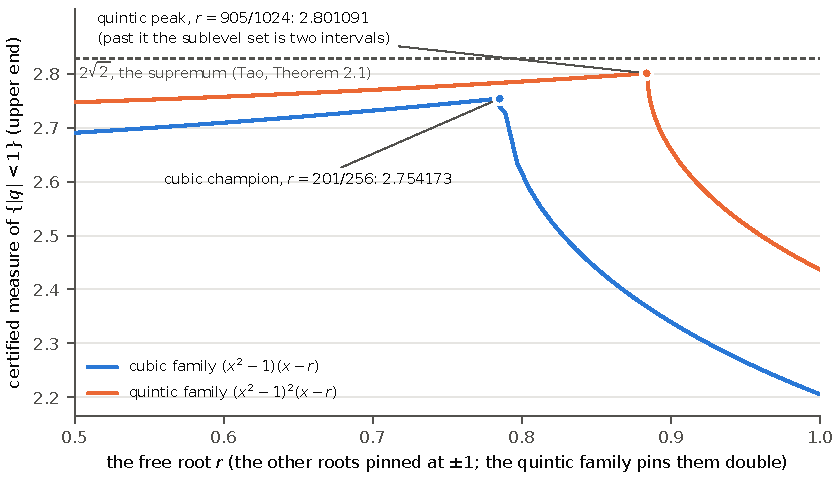
\includegraphics[width=\linewidth]{fig/erdos1038-sup-curves.pdf}
\caption{The two families against the free root $r$: $\CurvePoints$ certified enclosures
recomputed for this document (the plotted value is the upper end; widths are far below the
resolution of the picture). The quintic family is drawn at step $1/128$ and, between
$r=\FineFrom$ and $\FineTo$, at step $\FineStep$. Both families reach their maximum where their
sublevel set is still one interval and descend as soon as it splits.}\label{fig:curves}
\end{figure}

The descent is steep but continuous, as Lemma~\ref{lem:cont} requires; the report page's
description of it as a discontinuous drop is corrected here. The mechanism is visible in the
certified run structure: up to $r=\SplitBeforeR$ the quintic sublevel set is one interval
and the measure is $\SplitBeforeV$; at $r=\SplitAfterR$ a gap $[\SplitGapLo,\SplitGapHi]$ of
width $\SplitGapWidth$ has opened inside it and the measure is $\SplitAfterV$; by
$r=\FineLastR$ the gap is $\FineLastGapWidth$ wide. A local maximum of $\abs{q_r}$ inside the
interval has crossed the level $1$; when such a maximum is nondegenerate the excluded interval
has width of order $(r-r^*)^{1/2}$, which is the shape of the curve past each champion. At
$r=1$ the cubic family measures $\CubicEndV$ and the quintic $\QuinticEndV$.

\section{The thirty decimals of the infimum constant}\label{sec:decimals}

\subsection{What is defined, and what is checked}

Appendix~A of \cite{DPT} defines, with $\Lambda(y)=\log\frac{1+y}{1-y}$,
$p(q)=\log\frac{2}{1-q^2}/\Lambda(q)$ and $X_q(y)=\frac{2q^2-1-y^2}{1-y^2}$, the functions
$F_R(q,u)=\Lambda(u)-p(q)\log\frac{q+u}{q-u}$, $F_L(q,v)=\Lambda(v)-p(q)\log\frac{q+v}{v-q}$
and a third equation $K(q,u,v)$ built from them and from the displayed derivatives
(A.4)--(A.6); the extremal triple is the zero of $F=(F_R,F_L,K)$ inside the box $B_*$ of
radius $\RadiusB$ about centres $(q_0,u_0,v_0)$ printed to $\CentreDecimals$ decimals
(Table~\ref{tab:centres}), and $D=r^*-z^*$ with $r^*=X_{q^*}(u^*)$, $z^*=X_{q^*}(v^*)$. The
manuscript proves existence by a scalar intermediate-value argument on faces of $B_*$ and
ships Arb and SymPy certificates of its own \cite{DPT}.

\begin{table}[h]\centering\small
\begin{tabular}{lll}\toprule
centre & printed in (A.9) & certified expansion\\\midrule
\CentreRows
\bottomrule\end{tabular}
\caption{The box centres of the manuscript against the certified enclosures, which are thin to
$40$ decimals; the printed centres are the first $\CentreDecimals$ decimals of the zero.}\label{tab:centres}
\end{table}

The verifier, \texttt{verify.js} (its path is given in the Reproduction section), was written
against the manuscript on 4 August 2026 and filed on the authors' repository the next day
\cite{Pipeline5}; it is kept byte-identical and re-run, staged against this repository's
interval toolkit, at every build of the report page and for this document ($\VerPassed$ checks,
$\VerFailed$ failed, $\VerMutations$ mutation controls rejected, $\VerMs$\,ms). It executes no
line of the authors' code and takes no number from it except the claims under audit and the
centres of (A.9), which are part of the claim. One implementation of $F$ with forward-mode
automatic differentiation runs over two backends: outward-rounded IEEE-754 double intervals
with the interval logarithm of the \texttt{eqcert} toolkit \cite{Moore66}, and a fixed-point
BigInt interval layer at quantum $10^{-48}$ with directed rounding, the logarithm by the
$\operatorname{atanh}$ series after an exact power-of-two normalisation with an explicit tail
bound. The checks, in order:
\begin{enumerate}
\item the automatic derivatives overlap the manuscript's displayed closed forms (A.4)--(A.6);
\item the face inequalities (A.12)--(A.14) hold on $I_*=q_0\pm\RadiusI$ and the $u$, $v$ faces of
$B_*$, in a first-order mean-value form $F(m)+J(B)(B-m)$ --- the $F_R$ faces evaluate to an
interval between \FaceRLo\ and \FaceRHi\ and to its negative, the $F_L$ faces to intervals
between \FaceLLo\ and \FaceLHi\ in absolute value, so close to zero that naive interval
evaluation over the printed radii is too wide to decide the sign;
\item the interval Krawczyk operator \cite{Krawczyk69} contracts in $\KrawczykRounds$ round with
radius \KrawczykRad, proving existence and local uniqueness of the zero; this is a different
route from the manuscript's, and $B_*$ lies inside the uniqueness box, so the two triples are
the same zero;
\item iterating $X\leftarrow K(X)\cap X$ in the fixed-point layer refines the enclosure to widths
\WidthQ, \WidthU, \WidthV in $q,u,v$, with the first high-precision image re-checked to
land in the interior; the refined $q^*$ lies in $I_*$ and the triple in $B_*$, which is
Lemma~A.1 of \cite{DPT};
\item the derived constants are enclosed and every printed expansion is compared digit for
digit (Table~\ref{tab:claims}): a printed string matches as a \emph{truncation} if the enclosure
pins the truncation at that many decimals and it equals the string, as a \emph{rounding} if the
same holds for the half-up rounding;
\item four mutation controls must be rejected: the last printed digit of $D$ bumped
($\ldots125\to\ldots126$); the sign inside $K$ flipped, after which $F_3$ at the certified triple
is $\MutTwo$, not zero; the box shifted by $10^{-10}$ in $q$, where $F_R$ is \MutThree away
from zero; and the constant $2$ inside $p(q)$ perturbed to $2.000000001$, which moves $F_R$ at
the triple to \MutFour.
\end{enumerate}

\begin{table}[h]\centering\small
\resizebox{\linewidth}{!}{%
\begin{tabular}{llllc}\toprule
constant & page & printed in \cite{DPT} & certified expansion & matches as\\\midrule
\ClaimRows
\bottomrule\end{tabular}}
\caption{Every decimal expansion the manuscript prints for its extremal constants, against the
certified enclosures (thin to $40$ decimals; shown to three decimals past the printed length).
Nine match as truncations; the thirty-decimal headline $D$ matches as a half-up rounding.}\label{tab:claims}
\end{table}

\subsection{The thirtieth decimal}

The headline value on page~2 of \cite{DPT} is correct to under $5\times10^{-31}$: it is the
half-up rounding at thirty decimals of the certified expansion,
\[
\begin{aligned}
\text{printed (page 2):}\quad & \DPrintedThirty\ldots\\
\text{certified:}\quad & \DTwentyNine\,\DExpansionTail\ldots
\end{aligned}
\]
Read as an expansion prefix, which a trailing ellipsis conventionally promises, its last digit
differs from the expansion's ($\DPrintedLastDigit$ printed, $\DExpansionThirtieth$ in the
expansion). This is a presentation detail, not an error in the mathematics, and it is the kind
of detail only digit-level certified arithmetic can see; the same half-unit class is the benign
end of the failure taxonomy of the repository's audit of Erd\H{o}s \#852 \cite{Repo}. The
enclosures sit more than $\MarginDecades$ decades inside the box the manuscript's Lemma~A.1
asks for, which is what makes the printed decimals decidable rather than merely consistent.

\section{What is not claimed}\label{sec:notclaimed}

\begin{itemize}
\item \emph{The supremum theorem is not ours.} $\sup_\mu\meas{\{U_\mu<0\}}=2\sqrt2$ over all
probability measures on $[-1,1]$, with the two-atom measure as the only case of equality, is
Theorem~2.1 of \cite{TaoNotes}; for polynomials the value is attributed to \cite{El66,El68} in
\cite{DPT}. The certificates of Theorems~\ref{thm:odd} and~\ref{thm:even} neither use nor
replace it, and for even degrees their upper end is weaker than it. Degrees $1$ and $2$ are not
in the record (degree $1$ is the trivial measure $2$).
\item \emph{Degrees beyond $\MaxDegree$ are not decided.} Degree $\RefusedDegree$ is refused on
its budget; nothing is asserted about it or about any higher degree. The ladder is compute-bound,
not idea-bound, but that is a conjecture about the instrument and is not certified.
\item \emph{The equality case is not characterised by the certificates.} That the witness is
the only maximiser at even degrees follows from \cite{TaoNotes}, not from the localisation.
\item \emph{The landscape is data.} The cubic champion and the quintic peak are certified
values of explicit polynomials, hence certified lower bounds on $\sup_3$ and $\sup_5$; that they
are the maxima of their families is not certified (the grids are finite), and no lower witness
for degree $7$ is in the record.
\item \emph{The infimum is not decided here.} Proposition~\ref{prop:dec} verifies the
definition of $D$ and its printed digits. The extremality proof of \cite{DPT}, the other two
proof claims, the manuscript's own Arb and SymPy certificates (read for scope only) and its
AI-use chronology were not audited. The unconditional bracket on the infimum is the companion
paper's \cite{Companion}.
\item \emph{Nothing here is peer-reviewed.} The results are machine-derived; the repository
re-derives every number at every build, and refutations are invited.
\end{itemize}

\cmrepro{The records, the instruments and the commands, in the repository \cite{Repo} at
commit \texttt{\RepoCommit}:}
\begin{itemize}
\item \texttt{node tools/run-sublevel-campaign.js}\\
writes the supremum record \texttt{certs/sublevel-tao179.json} (about \RecMinutes\ minutes, most
of it the refused degree); the instrument is \texttt{instruments/sublevel/} (\texttt{measure.js},
\texttt{bound.js}, \texttt{battery.js}).
\item \texttt{node instruments/sublevel/battery.js}\\
re-proves degrees $3$ and $4$ and fires the three controls in well under a second.
\item \texttt{node tools/build-report-erdos1038-sup.js}\\
rebuilds the report page (\url{https://carlostoledo.co/reports/erdos1038-sup.html}),
re-certifying the witness, the calibrations and both family curves.
\item \texttt{node tools/build-report-lemniscate.js}\\
re-runs the thirty-decimal verifier, kept byte-identical at\\
\texttt{legacy/research/challenges/lane/laneb-lemniscate/verify.js},\\
against \texttt{instruments/interval} and rebuilds the verification page\\
\url{https://carlostoledo.co/reports/verify-lemniscate.html};\\
the earlier audit page is \url{https://carlostoledo.co/reports/claim-lemniscate.html}.
\item \texttt{node tools/paper-numbers/erdos1038-sup.js}\\
writes the macros of this document, the curve points of Figure~\ref{fig:curves} and the figure
itself, running the battery and the verifier live and refusing when a record no longer supports
a sentence; \texttt{node tools/build-paper-tex.js erdos1038-sup} compiles it.
\end{itemize}

\begin{thebibliography}{99}
\bibitem{EHP58} P.~Erd\H{o}s, F.~Herzog, G.~Piranian, Metric properties of polynomials, J.\ Analyse Math.\ 6 (1958), 125--148.
\bibitem{Po61} Ch.~Pommerenke, On metric properties of complex polynomials, Michigan Math.\ J.\ 8 (1961), 97--115.
\bibitem{El66} \'A.~Elbert, \"Uber eine Vermutung von Erd\H{o}s betreffs Polynome I, Studia Sci.\ Math.\ Hungar.\ 1 (1966), 119--128; as cited in \cite{DPT}.
\bibitem{El68} \'A.~Elbert, \"Uber eine Vermutung von Erd\H{o}s betreffs Polynome II, Studia Sci.\ Math.\ Hungar.\ 3 (1968), 299--324; as cited in \cite{DPT}.
\bibitem{Er76} P.~Erd\H{o}s, Extremal problems on polynomials, in: Approximation Theory II, Academic Press, 1976, 347--354; as cited in \cite{DPT}.
\bibitem{Bloom1038} T.~F.~Bloom, Erd\H{o}s Problem \#1038, \url{https://www.erdosproblems.com/1038}, accessed 2026-10-01 (page last edited 11 January 2026).
\bibitem{Tao179} T.~Tao, ``Beat the AI'' on \#1038, \texttt{teorth/erdosproblems} issue 179, \url{https://github.com/teorth/erdosproblems/issues/179}, 16 December 2025.
\bibitem{Forum1038} Erd\H{o}s Problems forum, thread 1038, \url{https://www.erdosproblems.com/forum/thread/1038}: T.~Tao, write-up completing the proof that the supremum is $2\sqrt2$ (post 2337, 21 December 2025), and the confirmations of N.~Sothanaphan and jspier (posts 2344 and 2348, 21 December 2025); accessed 2026-10-01.
\bibitem{TaoNotes} T.~Tao, Superlevel sets of logarithmic potentials, unpublished notes, 27 December 2025, \url{https://terrytao.wordpress.com/wp-content/uploads/2025/12/erdos-1038-2.pdf}.
\bibitem{Claims1038} Erd\H{o}s Problems, proof claims for \#1038, \url{https://www.erdosproblems.com/forum/thread/1038/proof-claims}, accessed 2026-10-01.
\bibitem{DPT} T.~Darvas, B.~Peng, R.~Tao, A solution to a problem of Erd\H{o}s--Herzog--Piranian, manuscript, 15 July 2026, 29 pp., \url{https://github.com/Pengbinghui/pipeline-math} (\texttt{papers/erdos1038/Erdos\_1038.pdf}); files at \url{https://osf.io/d6uq5/}.
\bibitem{Pipeline5} C.~Toledo, independent Krawczyk-route confirmation of Appendix A, issue 5 of \texttt{Pengbinghui/pipeline-math}, 5 August 2026, \url{https://github.com/Pengbinghui/pipeline-math/issues/5}.
\bibitem{Companion} C.~Toledo, Certified bounds for Erd\H{o}s problem \#1038, and a tail-free forcing argument, cert-machine pre-paper, September 2026, \url{https://carlostoledo.co/paper/erdos1038-inf.pdf}.
\bibitem{Repo} C.~Toledo, cert-machine: independent exact certification of machine-generated mathematics, repository, \url{https://github.com/carlostoledo1891/cert-machine}, concept DOI 10.5281/zenodo.22225860.
\bibitem{Krawczyk69} R.~Krawczyk, Newton-Algorithmen zur Bestimmung von Nullstellen mit Fehlerschranken, Computing 4 (1969), 187--201.
\bibitem{Moore66} R.~E.~Moore, Interval Analysis, Prentice-Hall, 1966.
\bibitem{BPR06} S.~Basu, R.~Pollack, M.-F.~Roy, Algorithms in Real Algebraic Geometry, 2nd ed., Springer, 2006.
\end{thebibliography}

\end{document}
